\normalfalse \difficiletrue \tdifficilefalse
\correctiontrue

%\UPSTIidClasse{11} % 11 sup, 12 spé
%\newcommand{\UPSTIidClasse}{11}

\exer{Suspension automobile  $\star\star$ \label{C1:05:55}}
\setcounter{numques}{0}
\UPSTIcompetence[2]{B2-14}
\UPSTIcompetence[2]{C1-05}
\index{Compétence B2-14}
\index{Compétence C1-05}
\index{PFS}
\index{Suspension automobile}
\ifcorrection
\else
\textbf{Pas de corrigé pour cet exercice.}
\fi

\ifprof
\else
On s'intéresse à la liaison entre l'axe de la toue et le châssis du véhicule. Les notations adoptées seront les suivantes : $F^a_{C}$ (respectivement $F^r_{C}$, $F^x_{C}$) désignera la composante suivant $\vect{a}$ (respectivement $\vect{r}$, $\vect{x}$) de l'effort extérieur exercé en $C$. On procédera de même pour le point $D$. 
\begin{center}
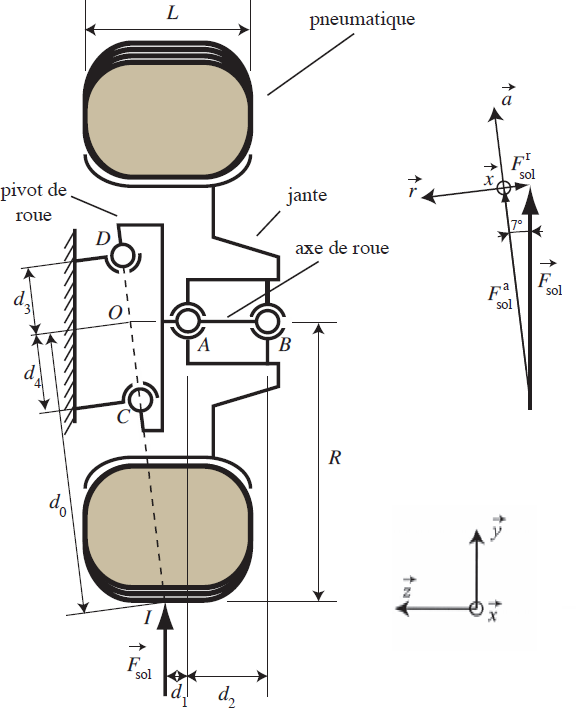
\includegraphics[width=\linewidth]{55_01}
\end{center}


\fi

\question{Réaliser le graphe d'analyse en faisant apparaître l'ensemble des actions mécaniques.}
\ifprof
\begin{center}
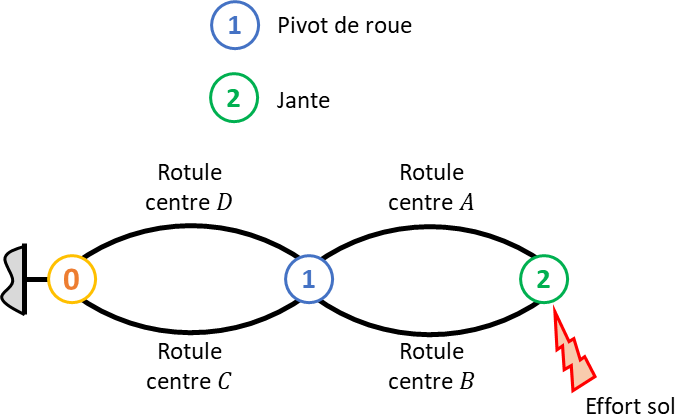
\includegraphics[width=10cm]{55_01_cor}
\end{center}

\else
\fi



\question{Peut-on résoudre complètement le système ? Pourquoi ?}
\ifprof
Calculons le degré d'hyperstatisme : 
\begin{itemize}
\item mobilités : $m=2$ (rotations autour de $\vect{a}$ et de $\vect{z}$);
\item inconnues statiques : $I_s = 3 \times 4 = 12$;
\item équations : $E_s = 2\times 6=12$. 
\item $h = m-E_s + I_s= 2 -12 + 12 = 2$.
\end{itemize}
On ne peut donc pas déterminer toutes les actions mécaniques. 

\else
\fi
\ifprof
\else
\begin{flushright}
\footnotesize{Corrigé  voir \ref{C1:05:55}.}
\end{flushright}%
\fi